\newcommand{\figModel}{
\begin{figure}[t]
    \centering
    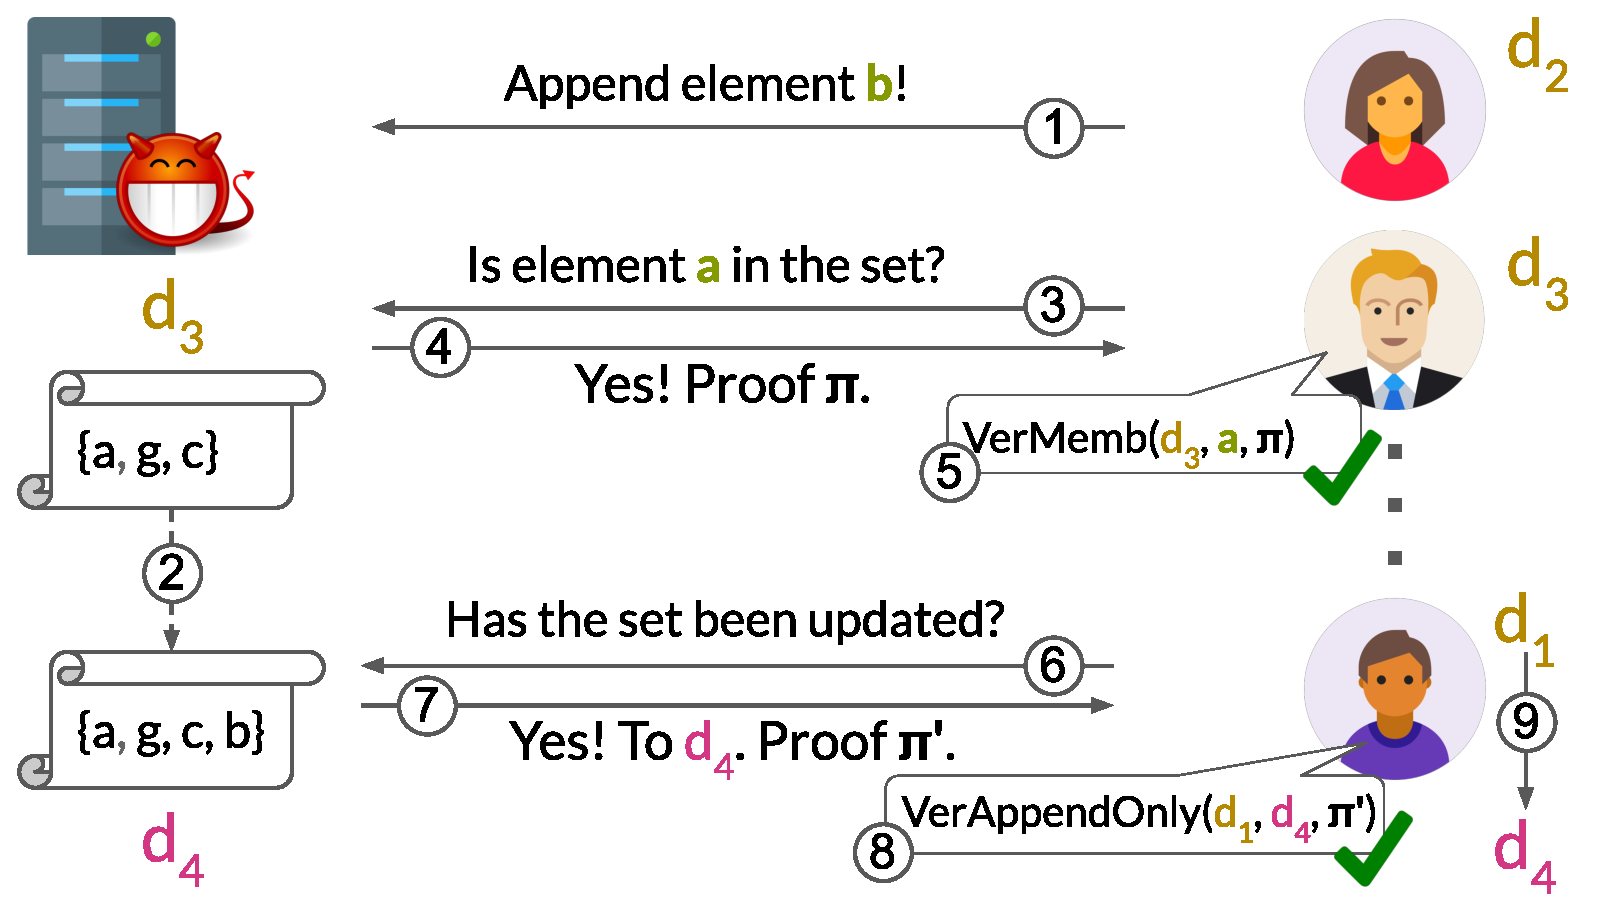
\includegraphics[width=.9\columnwidth]{figures-aad/model.pdf}
    %\vspace{-.5cm}
    \caption{
        Our model: a single malicious \textit{server} manages a \textit{set} and many \textit{clients} query the set.
        Clients will not necessarily have the digest of the latest set.
        The clients can (1) append a new element to the set, (2) query for an element and (3) ask for an updated digest of the set.
    }
    \label{f:model}
    %\vspace{-1.5em}
\end{figure}
}

\figModel

We begin by introducing a new primitive called an \textit{append-only authenticated set} (AAS).
An AAS is just a universal accumulator~\cite{LLX07} that supports subset witnesses and is fork-consistent.
We formalize the notion of an AAS in \cref{s:aas:defs} and instantiate it \textit{efficiently} from bilinear and RSA accumulators in \cref{s:aas:from-bilinear-acc} and in \cref{s:aas:from-rsa-acc}, respectively.
Then, in \cref{s:aad}, we slightly modify our AAS constructions to obtain \textit{append-only authenticated dictionaries} (AADs), which can be used to implement any transparency log~\cite{ELC16}.
Nonetheless, an AAS is useful in and of itself.
For example, it can be used for Revocation Transparency (RT)~\cite{Laurie15} to efficiently check the revocation status of certificates.

An AAS is a set of \textit{elements} managed by an \textit{untrusted server} and queried by \textit{clients}.
The server is the sole author of the AAS: it can append elements on its own and/or accept elements from clients.
% e.g., from History Tree paper: "Tamper-evident logs are fundamentally different: An untrusted logger is the sole author of the log and is responsible for both building and signing it.
% This is different from other models where elements might come from a \textit{trusted source} who signs them~\cite{two-party-ad,pads}.
Clients can check membership of elements in the set (see Steps 3-5 in \cref{f:model}).
Clients, also known as \textit{users}, are mutually-distrusting, potentially malicious, and do not have identities (i.e., no authorization or authentication).
Initially, the set starts out empty at \textit{version} zero, with new appends increasing its size and version by one.
Importantly, once an element has been appended to the set, it remains there forever: an adversary cannot remove nor change the element.
After each append, the server signs and publishes a new, small-sized \emph{digest} of the updated set (e.g., Step 2).

Clients periodically update their view of the set by requesting a new digest from the server (e.g., Step 6 and 7).
The new digest could be for an arbitrary version $j > i$, where $i$ is the previous version of the set (not just for $j = i+1$).
Importantly, clients always ensure the set remains \textit{append-only} by verifying an \textit{append-only proof} $\pi_{i,j}$ between the old and new digest (e.g., Step 8).
This way, clients can be certain the malicious server has not removed any elements from the set.
Clients will not necessarily have the latest digest of the set.
Finally, clients securely check if an element $k$ is in the set via a \emph{(non)membership proof} (e.g., Steps 3-5 in \cref{f:model}).

A malicious server can \emph{fork} clients' views~\cite{LKMS04}, preventing them from seeing each other's appends.
To deal with this, clients maintain a \textit{fork-consistent} view~\cite{LM07Beyond,LKMS04} of the set by checking append-only proofs.
As a consequence, if the server ever withholds an append from one client, that client's digest will forever diverge from other clients' digests.
To detect such \textit{forks}, clients can \textit{gossip}~\cite{CSP+15,STV+16,TD17,DPV+18} with one another about their digests.
This is crucial for security in transparency logs.

This model is the same as in history trees (HTs)~\cite{ht}, assuming only a gossip channel and no trusted third parties.
It also arises in encrypted web applications~\cite{mylar,verena,frientegrity}, Certificate Transparency (CT)~\cite{ct} and software transparency schemes~\cite{at,chainiac}.
Unlike the 2- and 3-party models~\cite{two-party-ad,pads,balloon}, there is no \textit{trusted source} that signs appends in this model.
A trusted source trivially solves the AAS/AAD problem as it can simply vouch for the data structure's append-only property with a digital signature.
Unfortunately, this kind of solution is useless for transparency logs~\cite{ct,Ryan2014,coniks}, which lack trusted parties.
